\documentclass[12pt,a4paper]{article}
\usepackage[utf8]{inputenc}
\usepackage[french]{babel}
\usepackage[T1]{fontenc}
\usepackage{hyperref}
\usepackage{geometry}
\usepackage{graphicx}
\geometry{hmargin=2.5cm,vmargin=2.5cm}

\begin{document}

% --- PAGE DE GARDE ---
\begin{titlepage}
    \centering
    
\includegraphics[width=0.3\textwidth]{logo-nanterre.png} \par % Ajout du logo
    {\large \textbf{Université Paris Nanterre}} \par
    \vspace{0.5cm}
    {\large Licence MIASHS L2} \par
    \vspace{2.5cm}
    {\huge \textbf{Rapport de projet informatique}} \par
    \vspace{1cm}
    {\Large \textbf{Hexagone Météo}} \par
    \vspace{2.5cm}
    
    \textbf{Membres du groupe :} \par
    \vspace{0.5cm}
    \textbf{ANN Seyda Dieynaba} - n° Étudiant : 45016888
    \par
    \textbf{Hawa Coulibaly} - n° Étudiant : 45016021 \par
    
    \vspace{2cm}
    \textbf{Lien vers le dépôt GitHub (Public) :}\par
    \url{https://github.com/sdaann/projet_Meteo_L2} \par
    \vfill
    {\large Année universitaire 2025-2026} \par
\end{titlepage}

% --- TABLE DES MATIÈRES ---
\newpage
\renewcommand{\contentsname}{Table des matières}
\tableofcontents % C'est ici que LaTeX va lister tout ce qui est écrit plus bas
\vfill
\centering 2 \par
\newpage

% --- SECTION 1 ---
\section{Introduction}

Le projet \textbf{Hexagone Météo} s'inscrit dans le cadre de l'unité d'enseignement informatique de la Licence 2 MIASHS à l'Université Paris Nanterre. Ce projet consiste en la conception et la réalisation d'une application web dynamique dédiée à la météorologie nationale française. 

L'enjeu principal de ce travail est de démontrer notre capacité à manipuler des données issues d'API externes et à les restituer de manière ergonomique et interactive pour l'utilisateur final. Le site permet non seulement de consulter le temps actuel, mais aussi d'accéder à des prévisions détaillées sur 24 heures et sur une période de 7 jours.

Les points forts de l'application incluent :
\begin{itemize}
    \item \textbf{Exploitation de données massives :} Récupération et traitement de flux JSON en temps réel via l'API \textit{WeatherAPI}.
    \item \textbf{Analyses Statistiques :} Suivi des consultations par ville stockées dans des fichiers CSV, permettant de générer dynamiquement un histogramme de fréquentation à l'aide de la bibliothèque graphique GD de PHP.
    \item \textbf{Personnalisation :} Utilisation de cookies pour mémoriser la dernière recherche de l'utilisateur et géolocalisation par adresse IP pour une expérience contextuelle.
    \item \textbf{Contenus Multimédia :} Intégration de l'image du jour (APOD) de la NASA pour enrichir l'aspect visuel et technique du site.
\end{itemize}

Ce rapport détaille les choix technologiques effectués, l'architecture du code, les difficultés rencontrées lors du passage à PHP 8.3, ainsi que la répartition du travail au sein de notre équipe.

\vfill
\centering 3 \par 
\newpage

% --- SECTION 2 ---
\section{Environnement de travail}

La réalisation du projet \textbf{Hexagone Météo} a nécessité la mise en place d'un environnement de développement complet, allant de la rédaction du code source jusqu'au déploiement sur serveur distant. Cet écosystème nous a permis de garantir la cohérence des données et la gestion des versions du site.

\subsection{Outils de développement et logiciels}
\begin{itemize}
    \item \textbf{Visual Studio Code (VS Code) :} Cet éditeur de texte a été notre outil principal pour le développement. Grâce à ses extensions PHP et son terminal intégré, nous avons pu coder les scripts côté serveur et les interfaces HTML/CSS avec une grande efficacité.
    \item \textbf{FileZilla :} Ce client FTP a été indispensable pour transférer nos fichiers locaux (scripts PHP, images, fichiers CSV) vers le serveur de production. Il nous a permis de gérer l'arborescence des dossiers directement sur l'hébergeur.
    \item \textbf{Navigateurs Web (Chrome / Firefox) :} Utilisés pour le test des interfaces et le débogage grâce aux outils de développement intégrés (Console, Inspecteur réseau).
\end{itemize}

\subsection{Hébergement et Serveur}
\begin{itemize}
    \item \textbf{Alwaysdata :} Le site est hébergé sur cette plateforme. Nous avons configuré l'environnement pour supporter \textbf{PHP 8.3}, ce qui nous a permis d'utiliser les dernières fonctionnalités du langage tout en nous confrontant aux nouvelles exigences de sécurité et de rigueur syntaxique.
    \item \textbf{Gestion des données :} Le serveur gère le stockage des statistiques de consultation via des fichiers CSV situés dans le répertoire \texttt{ressources/}.
\end{itemize}

\subsection{Gestion de version et collaboration}
\begin{itemize}
    \item \textbf{GitHub :} L'intégralité du code source est hébergée sur un dépôt public GitHub. Cela a permis une sauvegarde sécurisée du projet et une traçabilité des modifications effectuées sur les fichiers clés comme \texttt{function.inc.php} ou \texttt{prevision.php}.
    \item \textbf{LaTeX (Overleaf) :} Pour la rédaction du présent rapport, garantissant une mise en page structurée et professionnelle conforme aux attentes universitaires.
\end{itemize}

\vfill
\centering 4 \par
\newpage
% --- SECTION 3 ---
\section{Description du projet et objectifs}

Notre projet a été conçu comme une plateforme centralisée pour l'information météorologique en France. Au-delà d'une simple consultation de température, l'objectif était de créer un outil complet intégrant des données en temps réel, des statistiques de fréquentation et des contenus scientifiques.

\subsection{Objectifs principaux}
\begin{itemize}
    \item \textbf{Accessibilité :} Permettre à tout utilisateur de trouver rapidement la météo de sa commune grâce à une navigation intuitive par régions et départements (via une carte interactive).
    \item \textbf{Précision des données :} Garantir la fiabilité des informations en utilisant des flux de données professionnels (WeatherAPI) mis à jour en temps réel.
    \item \textbf{Analyse et Transparence :} Offrir une vue d'ensemble sur l'activité du site via une page de statistiques accessible à tous, illustrant les tendances de recherche des utilisateurs.
\end{itemize}

\subsection{Fonctionnalités détaillées du site}
Le site s'articule autour de plusieurs services clés :
\begin{itemize}
    \item \textbf{Système de recherche géographique :} Une navigation structurée permettant de filtrer les villes par région, puis par département, facilitant l'accès aux données locales.
    \item \textbf{Tableaux de prévisions complets :} Affichage des températures, de l'humidité, de la pression atmosphérique, de la vitesse du vent et des probabilités de pluie pour les 24 prochaines heures et les 7 jours à venir.
    \item \textbf{Analyse du profil visiteur :} Le site identifie automatiquement le \textbf{navigateur} utilisé par l'internaute et comptabilise le \textbf{nombre total de visites} via un compteur persistant stocké sur le serveur.
    \item \textbf{Dynamisme de l'accueil :} À chaque chargement, une \textbf{image aléatoire} est sélectionnée dans le répertoire de photos pour rendre l'interface plus vivante et variée.
    \item \textbf{Confort visuel (Mode Sombre) :} Intégration d'un mode sombre (Dark Mode) permettant d'adapter l'interface aux préférences de l'utilisateur pour une lecture plus agréable.
    \item \textbf{Module NASA APOD :} Une section affiche l'image astronomique du jour fournie par la NASA, démontrant notre capacité à croiser différentes sources d'API.
\end{itemize}
\vfill
\centering 5 \par
\newpage

% --- SECTION 4 ---
\section{Bibliothèques, Outils et technologies}

Le développement de ce projet repose sur une pile technologique moderne, choisie pour sa robustesse et sa capacité à traiter des flux de données externes.

\subsection{Langages et Frameworks}
\begin{itemize}
    \item \textbf{PHP 8.3 :} Langage principal utilisé pour toute la logique métier, le traitement des API et la gestion des fichiers CSV. L'utilisation de cette version récente a imposé une rigueur accrue, notamment pour les fonctions d'échange de données.
    \item \textbf{HTML5 / CSS3 :} Utilisés pour structurer et mettre en forme l'application, incluant l'utilisation de variables CSS pour le mode sombre.
\end{itemize}

\subsection{Bibliothèques et APIs}
\begin{itemize}
    \item \textbf{Bibliothèque GD (PHP) :} Utilisée dans le script \texttt{generate\_histogramme.php} pour créer dynamiquement des images PNG représentant les statistiques de consultation.
    \item \textbf{WeatherAPI (JSON) :} Source principale des données météorologiques, offrant des prévisions précises via des requêtes asynchrones.
    \item \textbf{NASA APOD API :} Récupération de l'image astronomique du jour au format JSON.
\end{itemize}

\subsection{Formats d'échange de données}
\begin{itemize}
    \item \textbf{JSON :} Format privilégié pour la réception des données météo et spatiales, traité avec \texttt{json\_decode()}.
    \item \textbf{CSV :} Utilisé pour le stockage local des statistiques de villes et la base de données des départements/régions de France.
\end{itemize}

\vfill
\centering 6 \par
\newpage

% --- SECTION 5 (IMPORTANT POUR LES CONSIGNES IA) ---
\section{Utilisation de l'Intelligence Artificielle}

Conformément aux directives du projet, cette section détaille l'usage fait des outils d'intelligence artificielle lors de la conception et du développement d'Hexagone Météo.

\subsection{Comment l'IA nous a aidé}
L'IA a été utilisée comme un partenaire de programmation (pair programming) pour résoudre des points de blocage spécifiques :
\begin{itemize}
    \item \textbf{Mise en conformité PHP 8.3 :} L'IA nous a permis de diagnostiquer l'origine des erreurs de type \textit{"Deprecated"} sur les fonctions \texttt{fgetcsv()} et \texttt{fputcsv()}. Elle a aidé à comprendre que le paramètre \texttt{\$escape} devait désormais être explicitement déclaré pour éviter la corruption des flux binaires, notamment pour l'histogramme.
    \item \textbf{Débogage de l'affichage graphique :} En analysant le code de \texttt{generate\_histogramme.php}, l'IA a aidé à identifier que des messages d'avertissement textuels s'inséraient avant les headers de l'image, empêchant ainsi le rendu correct du PNG dans la page de statistiques.
    \item \textbf{Structuration LaTeX :} L'IA a facilité la conversion du prototype de rapport en un document LaTeX structuré, garantissant le respect des normes universitaires de Paris Nanterre.
\end{itemize}

\subsection{Fonctionnement de l'IA utilisée}
L'IA sollicitée pour ce projet est un modèle de langage à grande échelle (LLM). Son fonctionnement repose sur :
\begin{itemize}
    \item \textbf{L'architecture Transformer :} Elle utilise des mécanismes d'attention pour comprendre les relations contextuelles entre les mots ou les lignes de code.
    \item \textbf{La prédiction probabiliste :} À partir d'un contexte (notre code source PHP), elle prédit la suite logique la plus pertinente, qu'il s'agisse d'une correction syntaxique ou d'une explication conceptuelle.
    \item \textbf{Traitement multimodal :} Le modèle est capable d'analyser à la fois du code source brut, des images (captures d'écran d'erreurs) et des documents PDF de consignes.
\end{itemize}

\section{Travail réalisé et répartition}
Le projet a été mené de manière collaborative en distinguant les tâches suivantes :
\begin{itemize}
    \item \textbf{Front-end :} Création des interfaces HTML/CSS, mise en place du mode sombre et intégration de la carte interactive.
    \item \textbf{Back-end :} Développement des fonctions de récupération d'API (WeatherAPI, NASA), gestion des fichiers de cache JSON et traitement des compteurs de visite.
    \item \textbf{Statistiques :} Développement du module de génération d'histogrammes et gestion des bases de données CSV pour les villes consultées.
\end{itemize}

\vfill
\centering 7 \par
\newpage

% --- SECTION 6 ---
\section{Difficultés rencontrées}

Le développement du projet a été marqué par plusieurs défis techniques. La résolution de ces problèmes a été une étape clé de notre apprentissage, nous obligeant à approfondir nos connaissances sur le fonctionnement des serveurs web et des flux de données.

\subsection{Migration et compatibilité PHP 8.3}
La difficulté la plus importante est survenue lors du déploiement sur le serveur Alwaysdata. Contrairement à notre environnement local, le serveur distant utilise \textbf{PHP 8.3}, une version très stricte sur la syntaxe.
\begin{itemize}
    \item \textbf{Erreurs de dépréciation :} Les fonctions de traitement CSV (\texttt{fgetcsv} et \texttt{fputcsv}) généraient des messages d'avertissement car le paramètre d'échappement (\texttt{\$escape}) n'était pas explicitement défini. 
    \item \textbf{Corruption de l'histogramme :} Ces messages de texte s'inséraient dans le flux de données de l'image générée par \texttt{generate\_histogramme.php}. Cela rendait l'image illisible pour le navigateur, provoquant un affichage vide sur la page des statistiques.
    \item \textbf{Résolution :} Nous avons dû mettre à jour chaque appel de fonction dans \texttt{function.inc.php} pour inclure les paramètres par défaut \texttt{",", "\"", "\textbackslash\textbackslash"}.
\end{itemize}

\subsection{Gestion des headers et flux de sortie}
Une autre difficulté a été de garantir qu'aucun caractère (espace ou ligne vide) ne soit envoyé au navigateur avant l'image de l'histogramme. 
\begin{itemize}
    \item Nous avons découvert que l'inclusion de fichiers avec la balise fermante \texttt{?>} pouvait parfois envoyer des espaces invisibles.
    \item \textbf{Solution :} Nous avons supprimé les balises fermantes dans les fichiers \texttt{include} et utilisé \texttt{exit} après la génération de l'image pour stopper tout envoi de données supplémentaire.
\end{itemize}

\subsection{Consommation d'APIs hétérogènes}
L'intégration simultanée de \textit{WeatherAPI} et de l'API \textit{NASA APOD} a nécessité une gymnastique technique, car chaque API possède sa propre structure JSON. Il a fallu créer des fonctions de décodage robustes capables de gérer les cas où certaines données (comme la description de l'image NASA) étaient absentes.

\vfill
\centering 8 \par
\newpage

% --- SECTION 7 ---
\section{Bilan}

Le projet \textbf{Hexagone Météo} a représenté une étape charnière dans notre cursus MIASHS, nous permettant de passer de la théorie algorithmique à la mise en œuvre d'un service web complexe et interconnecté.

\subsection{Conclusion technique et scientifique}
Le bilan de cette réalisation est extrêmement positif. Nous avons réussi à stabiliser une architecture logicielle capable de traiter des flux de données hétérogènes (JSON pour la météo, CSV pour les statistiques locales) sous un environnement serveur exigeant (PHP 8.3 sur Alwaysdata). 

La résolution des problèmes de corruption de flux binaire pour l'histogramme nous a permis de comprendre l'importance cruciale de la gestion des \textit{headers} HTTP et de la pureté du code de sortie en PHP. Ce projet démontre qu'une application météo n'est pas qu'un simple affichage, mais un véritable système de gestion d'information qui doit rester performant et fiable malgré les évolutions des versions de langages.

\subsection{Compétences acquises}
Au-delà du code, ce projet nous a permis de développer des compétences clés :
\begin{itemize}
    \item \textbf{Ingénierie des données :} Capacité à parser, filtrer et mettre en cache des données API pour optimiser les temps de chargement.
    \item \textbf{Analyse statistique :} Conception d'outils de visualisation dynamique (histogrammes) à partir de données de fréquentation brutes.
    \item \textbf{Adaptabilité technologique :} Apprentissage de la maintenance corrective face aux évolutions de PHP et à la rigueur de l'hébergement mutualisé professionnel.
\end{itemize}

\subsection{Perspectives et évolutions}
Bien que le site réponde à 100\% au cahier des charges actuel, nous envisageons plusieurs axes d'amélioration pour le futur :
\begin{itemize}
    \item \textbf{Optimisation UX :} Intégration d'une carte vectorielle (SVG ou Leaflet.js) pour remplacer la carte actuelle, afin d'offrir une interactivité plus fluide lors de la sélection des régions.
    \item \textbf{Module Prédictif :} Utilisation des données historiques collectées dans nos fichiers CSV pour tenter de modéliser les tendances de recherche locales via un algorithme de recommandation.
    \item \textbf{Système de Cache avancé :} Mise en place d'une base de données SQL pour remplacer le stockage CSV si le volume de statistiques venait à croître de manière significative.
\end{itemize}

\vfill
\centering 9 \par
\newpage

% --- ÉTAPE 7 : BIBLIOGRAPHIE ET WEBOGRAPHIE ---
\newpage
\section{Bibliographie}
\begin{itemize}
    \item \textbf{[LAM94]} L. LAMPORT, \textit{LaTeX: A Document Preparation System}, Addison-Wesley, 2.e édition, 1994. (Source de référence pour la rédaction de ce rapport).
    \item \textbf{[PHP8]} Documentation officielle, \textit{PHP 8.3 Manual}, Edition en ligne.
\end{itemize}

\section{Webographie}
Voici les ressources numériques consultées pour le développement d'Hexagone Météo :
\begin{itemize}
    \item \textbf{WeatherAPI :} \url{https://www.weatherapi.com/} — Fournisseur des données météorologiques JSON.
    \item \textbf{NASA APOD API :} \url{https://api.nasa.gov/} — Récupération de l'image astronomique du jour.
    \item \textbf{Alwaysdata Support :} \url{https://help.alwaysdata.com/} — Documentation sur l'hébergement et la configuration de PHP 8.3.
    \item \textbf{W3Schools PHP :} \url{https://www.w3schools.com/php/} — Aide pour la manipulation des fichiers CSV et de la bibliothèque GD.
\end{itemize}

% --- ÉTAPE 8 : ANNEXES ---
\newpage
\section{Annexes}

\subsection{Exemple d'exécution du projet}
\section{Exemple d'exécution du projet}

Cette annexe présente le fonctionnement de l'interface utilisateur du site \textbf{Hexagone Météo} à travers différentes étapes de navigation.

\subsection{Navigation Géographique}
L'utilisateur commence par sélectionner une région sur la carte interactive (Figure \ref{fig:carte}), puis choisit son département et sa ville via des menus déroulants dynamiques.

\begin{figure}[h]
    \centering
    % Remplacez 'carte.png' par le nom de votre fichier sur Overleaf
    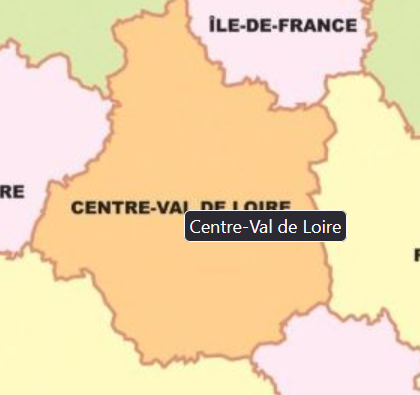
\includegraphics[width=0.4\textwidth]{carte.png} 
    \caption{Sélection de la région sur la carte de France.}
    \label{fig:carte}
\end{figure}

\begin{figure}[h]
    \centering
    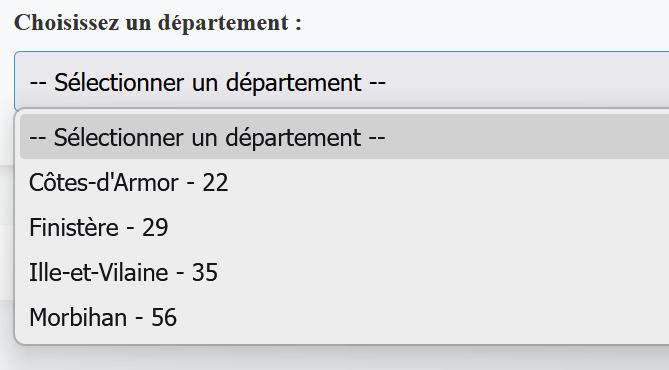
\includegraphics[width=0.6\textwidth]{departement.png}
    \caption{Menu de sélection des départements de la région choisie.}
\end{figure}

\begin{figure}[h]
    \centering
    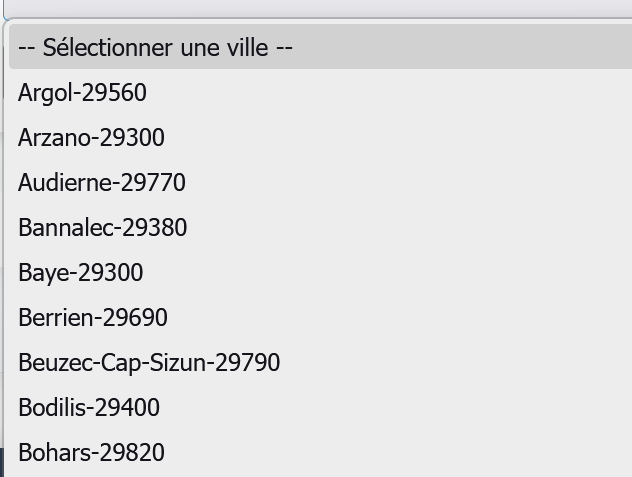
\includegraphics[width=0.6\textwidth]{ville.png}
    \caption{Liste filtrée des villes du département sélectionné.}
\end{figure}

\subsection{Affichage des Prévisions}
Une fois la ville sélectionnée (ici Audierne), le site affiche les conditions actuelles ainsi que les prévisions pour les jours suivants avec les horaires de lever et coucher du soleil.

\begin{figure}[h]
    \centering
    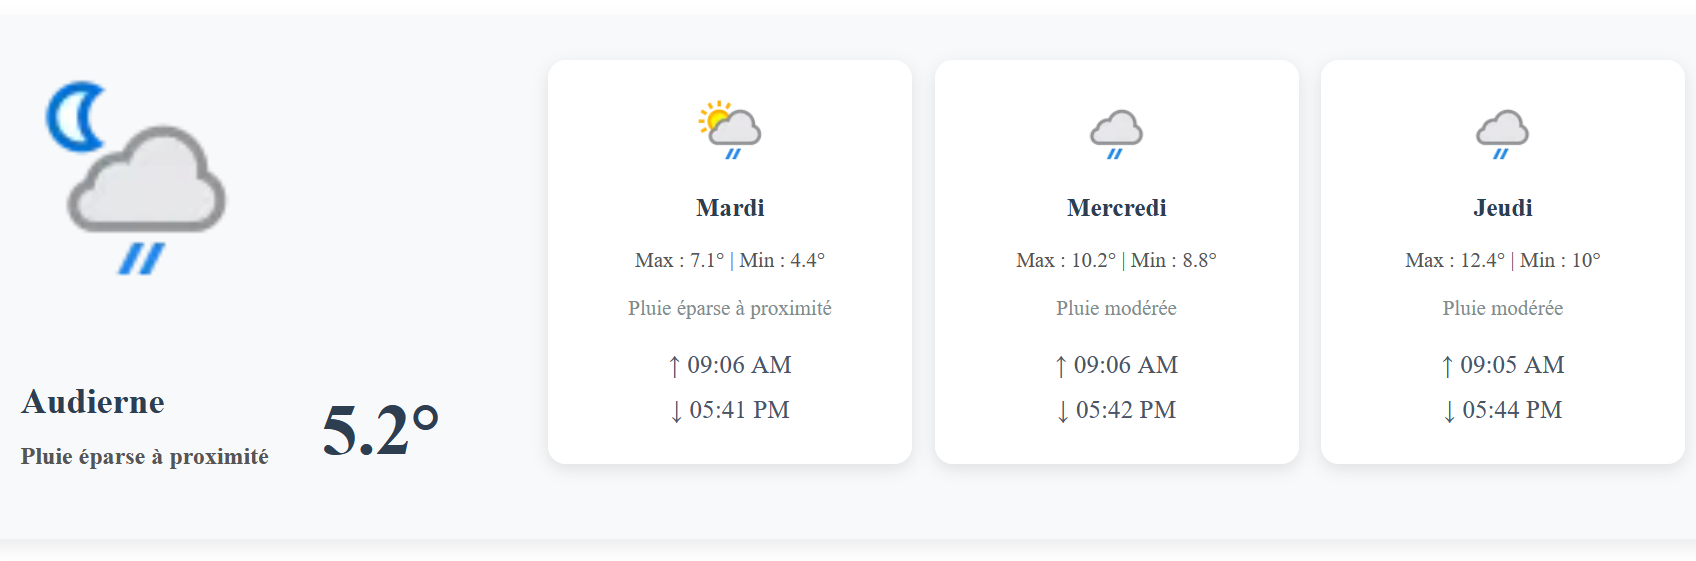
\includegraphics[width=0.9\textwidth]{meteo.png}
    \caption{Rendu final des prévisions météorologiques.}
\end{figure}

\subsection{Manuel utilisateur}
Pour utiliser le site, l'utilisateur doit :
\begin{enumerate}
    \item Se rendre sur l'URL Alwaysdata.
    \item Cliquer sur une région de la carte de France.
    \item Sélectionner un département puis une ville pour obtenir les prévisions.
    \item Consulter la page "Statistiques" pour voir l'historique des consultations globales.
\end{enumerate}

\vfill
\centering 10 \par % Page finale
\end{document}
% --- SECTION 10 ---
\section{Annexes}
\subsection{Exemple d'exécution du projet}
\vfill
\centering 3 \par

\end{document}